\documentclass[12pt]{article}

%=== Packages ===
\usepackage[margin=1in]{geometry}
\usepackage{amsmath,amssymb,amsthm}
\usepackage{mathtools}
\usepackage{natbib}
\usepackage[colorlinks=true,citecolor=blue,linkcolor=blue,urlcolor=blue]{hyperref}
\usepackage[capitalise,noabbrev]{cleveref}
\usepackage{booktabs}
\usepackage{enumitem}
\usepackage{graphicx}
\usepackage{tikz}
\usetikzlibrary{arrows.meta,positioning,decorations.markings}

%=== Theorem environments ===
\newtheorem{theorem}{Theorem}[section]
\newtheorem{proposition}[theorem]{Proposition}
\newtheorem{lemma}[theorem]{Lemma}
\newtheorem{corollary}[theorem]{Corollary}
\newtheorem{definition}[theorem]{Definition}
\newtheorem{remark}[theorem]{Remark}
\newtheorem{example}[theorem]{Example}
\newtheorem{axiom}{Axiom}

%=== Notation shortcuts ===
\newcommand{\R}{\mathbb{R}}
\newcommand{\E}{\mathbb{E}}
\newcommand{\Var}{\operatorname{Var}}
\newcommand{\Cov}{\operatorname{Cov}}
\newcommand{\Tr}{\operatorname{Tr}}
\newcommand{\calF}{\mathcal{F}}
\newcommand{\calH}{\mathcal{H}}
\newcommand{\calJ}{\mathcal{J}}
\newcommand{\calN}{\mathcal{N}}
\newcommand{\calR}{\mathcal{R}}
\newcommand{\calS}{\mathcal{S}}
\newcommand{\bone}{\mathbf{1}}

\title{The $(\rho, T)$ Framework:\\Six Axioms, One Phase Diagram, and the Deductive Structure\\of an Economic Free Energy Theory}
\author{Jon Smirl}
\date{February 2026 \\ \smallskip \textit{Working Paper}}

\begin{document}
\maketitle

\begin{abstract}
This paper consolidates a sequence of companion papers into a single deductive framework built on six axioms: constant returns to scale, scale consistency (which together force CES production), Shannon information constraints ($T$), timescale separation, Wright's Law learning, and directed input-output coupling.  From these six axioms, every result in the companion papers follows by mathematical derivation, with no additional assumptions.  The paper makes three contributions.  First, it states the axioms precisely, proves their independence, and maps the complete dependency structure: which results require which axioms.  Axioms 1--3 yield the static theory (free energy, effective curvature, crisis sequence, six classic economic results as special cases); adding Axiom 4 yields the multi-level hierarchy and eigenstructure bridge; adding Axiom 5 yields technology cycles; adding Axiom 6 yields business cycles; and all six together yield the self-referential closure where $\rho$ is endogenous and the system has no free structural parameters.  Second, it constructs the complete $(\rho, T)$ phase diagram---the single most important object in the framework---annotating all critical curves, bifurcation loci, oscillatory regions, and the limit-cycle attractor from the companion papers.  Third, it reconciles notational tensions across papers, compiles a unified inventory of 39 testable predictions organized by data requirement and specificity, and maps each theoretical result to its empirical counterpart in the applied papers (1--7).  This paper is intended to be read first: it provides the architecture that makes the companion papers legible as a unified theory rather than a collection of related results.
\end{abstract}

\textbf{JEL Codes:} B41, C02, D50, E32, O33

\textbf{Keywords:} axiomatic foundations, CES production, free energy, phase diagram, information temperature, unified theory, deductive structure

%=============================================================================
\section{Introduction}\label{sec:intro}
%=============================================================================

Between them, the companion papers derive business cycles from production technology, formalize Minsky's instability hypothesis, unify four classical cycle types as eigenfrequencies of a single operator, prove that the number of crises per technology wave is a topological invariant, and show that the economy self-organizes to its own critical curve.  But a reader encountering these papers in sequence faces two obstacles: the results were discovered in a different order than the logical structure requires, and each paper introduces notation calibrated to its specific domain rather than to the whole.

This paper removes both obstacles.  It presents the framework as it \emph{is}---a deductive system built on six axioms---rather than as it was discovered.  The reader who understands this paper can navigate any companion paper by locating it in the dependency graph (\cref{sec:dependencies}) and the phase diagram (\cref{sec:phase-diagram}).

\paragraph{The six axioms.}
The complete framework rests on:
\begin{enumerate}[nosep,label=\textbf{A\arabic*}:]
\item Constant returns to scale (homogeneity of degree one);
\item Scale consistency (aggregation is partition-invariant);
\item Shannon information constraints with temperature $T = 1/\kappa$;
\item Timescale separation across economic levels;
\item Wright's Law learning curves with elasticity $\alpha$;
\item Directed input-output coupling between sectors.
\end{enumerate}

Axioms A1--A2 together force CES production with complementarity parameter $\rho < 1$ \citep{smirl2026emergent}, making CES a theorem rather than an assumption.  The remaining axioms are \emph{independent}: no axiom is derivable from the others (\cref{sec:independence}).

\paragraph{Effective numbering convention.}
Since A1 and A2 always appear jointly in the results (CES requires both), the dependency tables, symbol table, and tier structure use a compound numbering with five effective axioms: \textbf{A1}~=~CES production (A1+A2 above), \textbf{A2}~=~Shannon information (A3 above), \textbf{A3}~=~Timescale separation (A4 above), \textbf{A4}~=~Wright's Law (A5 above), \textbf{A5}~=~Directed I/O (A6 above).  The six-axiom decomposition above is logically sharper; the five-axiom labeling is used in the symbol table (\cref{sec:symbols}), dependency table (\cref{sec:dependency-table}), tier diagram (\cref{sec:axiom-dependencies}), and open problems section (\cref{sec:open}).

The logical structure is cumulative: A1--A2 (effective) suffice for the static theory; each subsequent axiom unlocks a new layer of results.

\paragraph{Outline.}
\Cref{sec:axioms} states the axioms.  \Cref{sec:notation} establishes the unified notation, reconciling differences across papers.  \Cref{sec:phase-diagram} constructs the complete $(\rho, T)$ phase diagram.  \Cref{sec:dependencies} maps the deductive chain from axioms to results.  \Cref{sec:predictions} compiles the prediction inventory.  \Cref{sec:theory-application} maps theory to the applied papers.  \Cref{sec:open} identifies open problems.  \Cref{sec:conclusion} concludes.

%=============================================================================
\section{The Six Axioms}\label{sec:axioms}
%=============================================================================

\begin{axiom}[Constant Returns to Scale]\label{ax:crs}
Each productive unit $n$ aggregates $J_n \geq 2$ heterogeneous inputs via a function $F_n: \R_+^{J_n} \to \R_+$ that is homogeneous of degree one: $F_n(\lambda\mathbf{x}_n) = \lambda F_n(\mathbf{x}_n)$ for all $\lambda > 0$.
\end{axiom}

\begin{axiom}[Scale Consistency]\label{ax:nesting}
Aggregation is invariant to the level of coarse-graining: for any partition of inputs into blocks, computing $F_n$ directly gives the same result as first aggregating within blocks, then aggregating the block-level outputs.
\end{axiom}

These two axioms---constant returns and scale consistency---\emph{force} CES.  The Kolmogorov--Nagumo--Acz\'el theorem shows that the unique continuous, symmetric, strictly increasing aggregator satisfying both is the power mean \citep{smirl2026emergent}:
\begin{equation}\label{eq:ces}
F_n(\mathbf{x}_n) = \left(\frac{1}{J_n}\sum_{j=1}^{J_n} x_{nj}^{\rho_n}\right)^{1/\rho_n}, \qquad \rho_n \in (-\infty, 1).
\end{equation}
The elasticity of substitution is $\sigma_n = 1/(1-\rho_n)$, and the curvature parameter is $K_n = (1 - \rho_n)(J_n - 1)/J_n$.  CES is not a parametric assumption; it is the unique aggregation function compatible with multi-scale economic structure, in the same sense that the Gaussian is the unique limit of the Central Limit Theorem \citep{smirl2026emergent}.  The restriction $\rho < 1$ (complementarity, not perfect substitutability) is the sole substantive economic assumption: inputs are not interchangeable.

\begin{axiom}[Shannon Information Constraints]\label{ax:shannon}
Agents allocate inputs subject to a Shannon mutual information constraint:
\begin{equation}\label{eq:shannon}
I(\mathbf{x}; \boldsymbol{\theta}) \leq \kappa \quad \text{(nats)},
\end{equation}
where $\boldsymbol{\theta}$ is the vector of input qualities and $\kappa$ is channel capacity.  The \emph{information temperature} is $T = 1/\kappa$.
\end{axiom}

This is the rational inattention framework of \citet{sims2003}, parameterized by $T$ rather than $\kappa$.  Higher $T$ means less information capacity, coarser allocation, more entropy.  The key consequence: the equilibrium allocation maximizes the \emph{economic free energy}
\begin{equation}\label{eq:free-energy}
\calF(\mathbf{x}; \rho, T) = \Phi_{\mathrm{CES}}(\mathbf{x}; \rho) - T \cdot H(\mathbf{x}),
\end{equation}
where $\Phi = -\sum_n \log F_n$ is the CES potential and $H = -\sum_{nj} p_{nj}\log p_{nj}$ is Shannon entropy \citep{smirl2026free}.

\begin{axiom}[Timescale Separation]\label{ax:timescale}
The economy has $N$ levels with adjustment timescales $\tau_1 > \tau_2 > \cdots > \tau_N$, with adjacent ratios $r_k = \tau_k/\tau_{k+1} > r^*$ where $r^* \geq 2$ is the minimum ratio for the singular perturbation reduction to hold.
\end{axiom}

This is the standard assumption of multi-scale modeling \citep{kuehn2015}, applied to the economic observation that infrastructure changes more slowly than institutions, institutions more slowly than markets, and markets more slowly than financial prices.  Timescale separation enables the slow-manifold reductions that make the framework analytically tractable.

\medskip
\noindent\emph{Empirical calibration and approximation quality.}
Continuous wavelet transform (Morlet) analysis of US industrial production (FRED INDPRO, 1919--2025) identifies spectral peaks with median adjacent-peak separation ratio $2.1$ (IQR~$[1.84, 2.63]$, maximum $5.5$), yielding an effective hierarchy depth $N_{\mathrm{eff}} = 4$--$5$ across all decades (mean $4.5$, s.d.\ $1.0$) when $r^* = 2$ \citep{smirl2026complementary}.
At this empirically calibrated $r^* \approx 2$, the nearest-neighbor coupling topology (Paper 9b, Theorem~3.1(iv)) is an $O(1/r^*) \approx O(0.5)$ approximation: non-adjacent coupling terms are suppressed by a factor of $\sim 1/2$ relative to adjacent terms.
All qualitative results (activation threshold, ceiling cascade, damping cancellation) are robust to this correction; quantitative predictions (transition duration, spectral radius) carry $O(1/r^*)$ uncertainty.
The hierarchy is better understood as a \emph{wavelet multiresolution}---a continuous spectrum organized into approximately octave-spaced bands---rather than a cleanly separated discrete ladder.

\begin{axiom}[Wright's Law Learning]\label{ax:wright}
Cumulative production $Q_n$ reduces unit cost according to:
\begin{equation}\label{eq:wright}
c_n(Q_n) = c_{n,0} \cdot Q_n^{-\alpha_n}, \qquad \alpha_n \in (0, 1),
\end{equation}
where $\alpha_n$ is the learning elasticity.
\end{axiom}

Wright's Law is the most robust empirical regularity in the economics of technological change, verified across semiconductors, solar cells, batteries, aircraft, and dozens of other technologies \citep{wright1936,nagy2013}.  The learning elasticity $\alpha$ is a measurable physical constant of the production process.

\begin{axiom}[Directed Input-Output Coupling]\label{ax:io}
Sectors are coupled through a Leontief input-output matrix $\mathbf{A} = [a_{nm}]$ that is generically asymmetric: $\mathbf{A} \neq \mathbf{A}^\top$.  The decomposition $\mathbf{A} = \mathbf{S} + \mathbf{J}_A$ into symmetric ($\mathbf{S}$) and antisymmetric ($\mathbf{J}_A$) components satisfies $\|\mathbf{J}_A\|_F / \|\mathbf{S}\|_F > 0$.
\end{axiom}

This is an empirical statement about the structure of real input-output tables: supply chains are directed.  Steel feeds into automobiles but not conversely.  The antisymmetric component is not small---in US BEA tables, $\|\mathbf{J}_A\|_F / \|\mathbf{S}\|_F \approx 0.4$--$0.7$ \citep{smirl2026business}.

\subsection{Independence of the axioms}\label{sec:independence}

\begin{proposition}[Axiom independence]\label{prop:independence}
No axiom is derivable from the remaining five.
\end{proposition}

\begin{proof}[Proof sketch]
For each axiom, exhibit a model satisfying the others but violating it:
\begin{enumerate}[nosep]
\item \emph{Drop A1} (CRS): An economy with fixed costs (increasing returns at small scale) satisfies A2--A6 but violates homogeneity.
\item \emph{Drop A2} (Scale consistency): A translog production function satisfies A1, A3--A6 but violates partition invariance---the aggregate depends on how inputs are grouped.
\item \emph{Drop A3} (Shannon): A perfect-information economy ($T = 0$) satisfies A1--A2, A4--A6 but has no information constraints.  The free energy reduces to the CES potential without the entropy term.
\item \emph{Drop A4} (Timescale separation): A single-level economy satisfies A1--A3, A5--A6 but has no hierarchical structure.
\item \emph{Drop A5} (Wright's Law): A static-technology economy with fixed costs satisfies A1--A4, A6 but has no learning dynamics.
\item \emph{Drop A6} (Directed I/O): An economy with symmetric trade ($\mathbf{A} = \mathbf{A}^\top$) satisfies A1--A5 but produces purely dissipative dynamics with no oscillatory modes.
\end{enumerate}
\end{proof}

%=============================================================================
\section{Unified Notation}\label{sec:notation}
%=============================================================================

The companion papers developed organically, producing notational inconsistencies.  This section establishes the canonical notation.

\subsection{Resolving $T^*$}\label{sec:resolve-Tstar}

The critical temperature appears in two forms across the papers:
\begin{itemize}[nosep]
\item \textbf{Paper 10} (exact): $T^*_n = 2(J_n - 1)c_n^2 d_n^2 / K_n$, derived from the condition that the output loss from misallocation equals the complementarity premium.
\item \textbf{Papers 11--15} (leading-order): $T^*_n \approx K_n$, valid at the symmetric allocation with unit-normalized inputs.
\end{itemize}

\begin{definition}[Canonical critical temperature]\label{def:Tstar}
The critical temperature of sector $n$ is:
\begin{equation}\label{eq:Tstar}
T^*_n = \frac{(1-\rho_n)(J_n - 1)}{J_n} \cdot \frac{2\bar{x}_n^2}{\lambda_{\max}(-\nabla^2\Phi_n|_{\mathrm{sym}})^{-1}} = K_n \cdot \Theta_n,
\end{equation}
where $\Theta_n = 2\bar{x}_n^2 / \lambda_{\max}^{-1}$ is a normalization factor equal to 1 at the symmetric allocation with unit inputs.  Papers 11--15 work at $\Theta_n = 1$; Paper 10 retains the full expression.  No results conflict: the leading-order approximation $T^* \approx K$ is exact at symmetric equilibrium and correct to first order elsewhere.
\end{definition}

\subsection{Resolving $H$}\label{sec:resolve-H}

Two objects share the letter $H$:
\begin{itemize}[nosep]
\item $H(\mathbf{p}) = -\sum_j p_j \log p_j$: Shannon entropy of the allocation (Papers 8--10).
\item $\calH(\mathbf{x})$: the Hamiltonian of the port-Hamiltonian system (Papers 13--14).
\end{itemize}

\begin{definition}[Canonical notation]\label{def:H-notation}
We reserve:
\begin{itemize}[nosep]
\item $H$ for Shannon entropy;
\item $\calF = \Phi - T \cdot H$ for the economic free energy;
\item The port-Hamiltonian form uses $\calF$ as the Hamiltonian: $\dot{\mathbf{x}} = (\mathbf{J} - \mathbf{R})\nabla\calF$.
\end{itemize}
There is no separate ``Hamiltonian''---the free energy $\calF$ plays both roles.  The port-Hamiltonian system conserves $\calF$ along $\mathbf{J}$-flows (antisymmetric part) and dissipates $\calF$ along $\mathbf{R}$-flows (symmetric part).
\end{definition}

\subsection{Resolving gradient flow vs.\ port-Hamiltonian}\label{sec:resolve-dynamics}

Paper 12 uses gradient flow ($\dot{\mathbf{x}} = -\mathbf{L}\nabla\calF$).  Paper 14 uses port-Hamiltonian dynamics ($\dot{\mathbf{x}} = (\mathbf{J} - \mathbf{R})\nabla\calF$).  These are not alternatives---they are limits of a single system.

\begin{proposition}[Dynamics hierarchy]\label{prop:dynamics-hierarchy}
The full dynamics of the multi-sector economy are port-Hamiltonian:
\begin{equation}\label{eq:full-dynamics}
\dot{\mathbf{x}} = (\mathbf{J} - \mathbf{R})\nabla\calF.
\end{equation}
Three limiting cases:
\begin{enumerate}[nosep]
\item \textbf{Within-sector} ($\mathbf{J} = 0$): reduces to gradient flow $\dot{\mathbf{x}} = -\mathbf{R}\nabla\calF$.  This is Paper 12's framework.  No oscillations; monotone convergence.
\item \textbf{Infinite timescale separation} ($\varepsilon \to 0$): each level equilibrates instantly on its own slow manifold.  The effective dynamics are sequential gradient flows with no cross-level oscillations.  This is Paper 9b's framework.
\item \textbf{Finite timescale separation} ($\varepsilon > 0$): the antisymmetric coupling $\mathbf{J}$ from directed input-output linkages generates oscillatory modes.  This is Paper 14's framework.
\end{enumerate}
Gradient flow is the $\mathbf{J} = 0$ or $\varepsilon \to 0$ limit of the port-Hamiltonian system.  All results derived under gradient flow remain valid as the dissipative component of the full dynamics.
\end{proposition}

\subsection{Master symbol table}\label{sec:symbols}

\begin{center}
\small
\begin{tabular}{lll}
\toprule
Symbol & Meaning & Axiom origin \\
\midrule
$\rho_n \in (-\infty, 1)$ & CES complementarity parameter, sector $n$ & A1 \\
$\sigma_n = 1/(1-\rho_n)$ & Elasticity of substitution & A1 \\
$K_n = (1-\rho_n)(J_n-1)/J_n$ & Curvature parameter & A1 \\
$J_n$ & Number of inputs in sector $n$ & A1 \\
$F_n$ & CES aggregate output & A1 \\
$\Phi = -\sum_n \log F_n$ & CES potential (production difficulty) & A1 \\
$T = 1/\kappa$ & Information temperature & A2 \\
$H = -\sum p_j \log p_j$ & Shannon entropy of allocation & A2 \\
$\calF = \Phi - TH$ & Economic free energy & A1+A2 \\
$T^*_n \approx K_n$ & Critical temperature, sector $n$ & A1+A2 \\
$K_{\mathrm{eff}} = K(1-T/T^*)^+$ & Effective curvature under friction & A1+A2 \\
$\varepsilon_k = \tau_{k+1}/\tau_k$ & Timescale ratio between levels & A3 \\
$\alpha_n$ & Wright's Law learning elasticity & A4 \\
$Q_n(t) = \int_0^t I_n(s)\,ds$ & Cumulative investment & A4 \\
$\mathbf{R}$ & Dissipation matrix (symmetric, $\succeq 0$) & A1+A2 \\
$\mathbf{J}$ & Antisymmetric coupling matrix & A5 \\
$\zeta = r/\omega$ & Damping ratio & A2+A5 \\
$\bar{\rho}(t)$ & Economy-wide effective complementarity & A1 (endogenized by A4) \\
\bottomrule
\end{tabular}
\end{center}

%=============================================================================
\section{The Complete $(\rho, T)$ Phase Diagram}\label{sec:phase-diagram}
%=============================================================================

The $(\rho, T)$ plane is the fundamental state space of the framework.  Every equilibrium, every transition, every cycle, and every crisis can be located on it.  This section constructs the complete diagram by assembling features from all companion papers.

\subsection{The critical curve}\label{sec:critical-curve}

The most important object in the diagram is the critical curve:
\begin{equation}\label{eq:critical-curve}
T^*(\rho) = \frac{(1-\rho)(J-1)}{J} = K(\rho),
\end{equation}
a decreasing, convex curve from $T^* = (J-1)/J$ at $\rho = 0$ to $T^* \to \infty$ as $\rho \to -\infty$ and $T^* \to 0$ as $\rho \to 1$.  This curve separates:
\begin{itemize}[nosep]
\item \textbf{Below} ($T < T^*$): efficient regime.  The free energy landscape has a well-defined minimum; allocation exploits complementarity; all three roles of $K$ are active.
\item \textbf{Above} ($T > T^*$): breakdown regime.  The free energy landscape flattens; allocation degrades to uniform randomness; complementarity premium vanishes.
\end{itemize}

\subsection{The crisis sequence boundaries}\label{sec:crisis-boundaries}

Within the efficient regime, the three roles of curvature degrade at different rates as $T$ rises (Paper 10).  Define:
\begin{align}
T_{\mathrm{corr}}^*(\rho) &= T^*(\rho)/2, \label{eq:T-corr} \\
T_{\mathrm{super}}^*(\rho) &= T^*(\rho), \label{eq:T-super} \\
T_{\mathrm{strat}}^*(\rho) &= T^*(\rho) \cdot (1 + \delta), \quad \delta \ll 1, \label{eq:T-strat}
\end{align}
where:
\begin{enumerate}[nosep]
\item At $T = T_{\mathrm{corr}}^*$: correlation robustness has lost 75\% of its value (quadratic degradation $\propto (1 - T/T^*)^2$).  Diversification strategies fail.
\item At $T = T_{\mathrm{super}}^*$: superadditivity reaches zero (linear degradation $\propto (1 - T/T^*)$).  Complementary production ceases to outperform.
\item At $T = T_{\mathrm{strat}}^*$: strategic independence breaks.  Coordination collapses; this is the threshold event.
\end{enumerate}

The crisis sequence---financial crisis, then productive disruption, then governance breakdown---is the universal order of crossing these boundaries as $T$ increases at fixed $\rho$.  It is forced by the mathematics (quadratic degrades faster than linear) and independent of institutional detail.

\subsection{The oscillation boundary}\label{sec:oscillation-boundary}

The damping ratio $\zeta = r/\omega$ (Paper 14) determines whether the economy oscillates or converges monotonically.  In the $(\rho, T)$ plane, the boundary $\zeta(\rho, T) = 1$ separates:
\begin{itemize}[nosep]
\item \textbf{Underdamped region} ($\zeta < 1$): oscillatory dynamics, visible business cycles.  This region lies where within-sector dissipation $r$ is low relative to cross-sector antisymmetric coupling $\omega$.
\item \textbf{Overdamped region} ($\zeta > 1$): monotone convergence, no visible cycles.  This region lies where regulation or friction dominates coupling.
\end{itemize}

The Great Moderation (1984--2007) corresponds to the economy crossing from the underdamped to the overdamped region.  Financial deregulation increased effective within-sector dissipation $r$ by making markets more liquid and mean-reverting---deeper, faster-clearing markets absorb shocks that previously propagated as oscillatory modes (Paper 14, Theorem 8.1).

\subsection{The Perez limit cycle}\label{sec:limit-cycle}

With endogenous $\rho$ (Paper 15), the system traces a limit cycle $\Gamma$ in $(\rho, T)$ space.  The cycle orbits the critical curve $T^*(\rho)$, crossing it twice per period (entering and exiting crisis).  The four phases of the Perez technology cycle occupy the four quadrants of $\Gamma$ relative to its center:

\begin{center}
\begin{tikzpicture}[scale=1.2, >=Stealth]
% Axes
\draw[->] (-0.3,0) -- (5.5,0) node[right] {$\rho$};
\draw[->] (0,-0.3) -- (0,4.5) node[above] {$T$};

% Critical curve T*(rho) = (1-rho)*C, depicted as decreasing curve
\draw[thick, blue] plot[smooth, domain=0.3:4.8] (\x, {4.0/\x});
\node[blue, right] at (4.8, 0.95) {$T^*(\rho)$};

% Crisis sequence boundaries (dashed)
\draw[dashed, red!60] plot[smooth, domain=0.6:4.8] (\x, {2.0/\x});
\node[red!60, right, font=\footnotesize] at (4.5, 0.55) {$T^*_{\mathrm{corr}}$};

% Limit cycle (ellipse-like, tilted)
\draw[thick, black, decoration={markings, mark=at position 0.15 with {\arrow{>}}, mark=at position 0.4 with {\arrow{>}}, mark=at position 0.65 with {\arrow{>}}, mark=at position 0.9 with {\arrow{>}}}, postaction={decorate}]
  (1.5, 1.0) .. controls (1.0, 1.8) and (1.0, 2.8) .. (1.8, 3.2)
  .. controls (2.4, 3.5) and (3.2, 3.0) .. (3.5, 2.2)
  .. controls (3.7, 1.6) and (3.5, 0.8) .. (2.8, 0.6)
  .. controls (2.2, 0.4) and (1.7, 0.6) .. (1.5, 1.0);

% Phase labels
\node[font=\footnotesize] at (0.7, 1.5) {\textbf{I}};
\node[font=\footnotesize] at (1.2, 3.2) {\textbf{II}};
\node[font=\footnotesize] at (3.6, 2.8) {\textbf{III}};
\node[font=\footnotesize] at (3.8, 0.8) {\textbf{IV}};

% Phase legend
\node[font=\footnotesize, anchor=west] at (4.8, 4.0) {\textbf{I}: Installation};
\node[font=\footnotesize, anchor=west] at (4.8, 3.5) {\textbf{II}: Frenzy/Crisis};
\node[font=\footnotesize, anchor=west] at (4.8, 3.0) {\textbf{III}: Turning point};
\node[font=\footnotesize, anchor=west] at (4.8, 2.5) {\textbf{IV}: Deployment};

% Region labels
\node[font=\footnotesize, gray] at (3.0, 0.3) {Efficient};
\node[font=\footnotesize, gray] at (1.0, 3.8) {Breakdown};
\end{tikzpicture}
\end{center}

\begin{theorem}[Complete phase diagram]\label{thm:phase-diagram}
The $(\rho, T)$ phase diagram contains the following features, assembled from the companion papers:
\begin{enumerate}
\item \textbf{Critical curve} $T^*(\rho) = K(\rho)$ [Papers 9, 10]: separates efficient and breakdown regimes.
\item \textbf{Crisis sequence boundaries} $T_{\mathrm{corr}}^* < T_{\mathrm{super}}^* < T_{\mathrm{strat}}^*$ [Paper 10]: three parallel curves below $T^*$, marking the progressive failure of correlation robustness, superadditivity, and strategic independence.
\item \textbf{Damping ratio boundary} $\zeta(\rho, T) = 1$ [Paper 14]: separates underdamped (oscillatory) and overdamped (monotone) regions.
\item \textbf{Perez limit cycle} $\Gamma$ [Paper 15]: closed orbit around $T^*(\rho)$ traced by the endogenous $(\rho, T)$ dynamics, with period $\sim 25$--$50$ years.
\item \textbf{Self-organized critical attractor} [Paper 15]: the limit cycle $\Gamma$ orbits the critical curve, spending most time in the sub-critical region (slow drift) and brief time in the super-critical region (fast crisis).
\item \textbf{Winding number quantization} [Paper 13]: each complete orbit of $\Gamma$ around $T^*(\rho)$ contributes exactly one winding, giving a topologically protected integer crisis count.
\end{enumerate}
\end{theorem}

\subsection{Reading the diagram}\label{sec:reading}

The phase diagram encodes the answer to every qualitative question about economic dynamics:

\begin{itemize}[nosep]
\item \emph{Will this economy have business cycles?}  Check whether $(\rho, T)$ lies in the underdamped region ($\zeta < 1$).
\item \emph{How fragile is this economy?}  Measure the distance $T^*(\rho) - T$ from the current state to the critical curve.
\item \emph{Which crisis will come first?}  As $T$ rises, the first boundary crossed is $T_{\mathrm{corr}}^*$ (financial crisis).
\item \emph{Where are we in the Perez cycle?}  Locate $(\rho, T)$ on the limit cycle $\Gamma$.  Falling $\rho$ = installation; rising $\rho$ = deployment; crossing $T^*$ = turning point.
\item \emph{What does regulation do?}  Regulation increases $r$ (within-sector dissipation), shifting $\zeta$ upward.  This damps oscillations without moving the critical curve.
\item \emph{What does monetary policy do?}  Rate cuts lower $T$, moving the economy downward in the diagram.  But endogenous $\rho$-shift (Minsky trap) simultaneously moves the critical curve, partially offsetting the benefit.
\end{itemize}

%=============================================================================
\section{The Deductive Chain}\label{sec:dependencies}
%=============================================================================

\subsection{Axiom dependency graph}\label{sec:axiom-dependencies}

The results of the companion papers organize into five tiers, each requiring one additional axiom:

\begin{center}
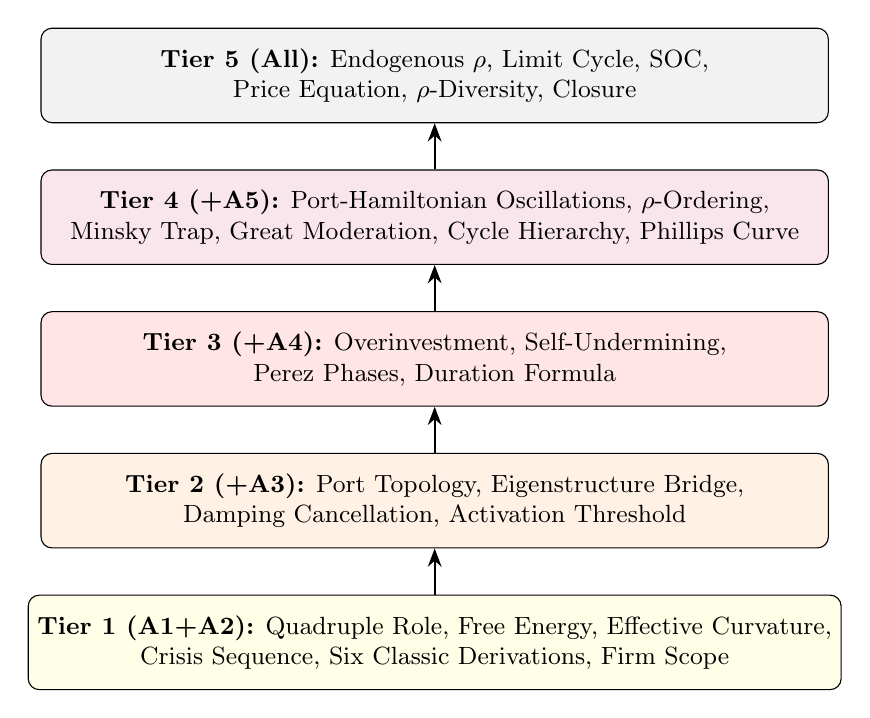
\begin{tikzpicture}[
  tier/.style={draw, rounded corners, minimum width=10cm, minimum height=1.2cm, align=center, font=\small},
  axiom/.style={draw, fill=blue!10, rounded corners, font=\small\bfseries, minimum width=1.8cm},
  >=Stealth
]

% Tiers
\node[tier, fill=yellow!10] (t1) at (0,0) {%
  \textbf{Tier 1 (A1+A2):} Quadruple Role, Free Energy, Effective Curvature,\\
  Crisis Sequence, Six Classic Derivations, Firm Scope};
\node[tier, fill=orange!10] (t2) at (0,1.8) {%
  \textbf{Tier 2 (+A3):} Port Topology, Eigenstructure Bridge,\\
  Damping Cancellation, Activation Threshold};
\node[tier, fill=red!10] (t3) at (0,3.6) {%
  \textbf{Tier 3 (+A4):} Overinvestment, Self-Undermining,\\
  Perez Phases, Duration Formula};
\node[tier, fill=purple!10] (t4) at (0,5.4) {%
  \textbf{Tier 4 (+A5):} Port-Hamiltonian Oscillations, $\rho$-Ordering,\\
  Minsky Trap, Great Moderation, Cycle Hierarchy, Phillips Curve};
\node[tier, fill=gray!10] (t5) at (0,7.2) {%
  \textbf{Tier 5 (All):} Endogenous $\rho$, Limit Cycle, SOC,\\
  Price Equation, $\rho$-Diversity, Closure};

% Arrows
\draw[->, thick] (t1) -- (t2);
\draw[->, thick] (t2) -- (t3);
\draw[->, thick] (t3) -- (t4);
\draw[->, thick] (t4) -- (t5);

\end{tikzpicture}
\end{center}

\noindent Additionally, the dynamical results (Paper 12: FDT, critical slowing, Onsager, Kramers, Jarzynski) require A1+A2+A3 and are Tier~2.  The conservation laws (Paper 13: Euler identity, permutation constraints, Crooks, winding number, Casimirs) span Tiers~2--4 depending on the specific result.

\subsection{Detailed dependency table}\label{sec:dependency-table}

\begin{center}
\small
\renewcommand{\arraystretch}{1.1}
\begin{tabular}{p{5.5cm}cccccp{1.5cm}}
\toprule
Result & A1 & A2 & A3 & A4 & A5 & Paper \\
\midrule
\multicolumn{7}{l}{\textit{Tier 1: Static foundation}} \\
Quadruple Role of $K$ & $\checkmark$ & & & & & 8 \\
Free energy $\calF = \Phi - TH$ & $\checkmark$ & $\checkmark$ & & & & 9 \\
Effective curvature $K_{\mathrm{eff}}$ & $\checkmark$ & $\checkmark$ & & & & 10 \\
Crisis sequence & $\checkmark$ & $\checkmark$ & & & & 10 \\
Akerlof, Myerson, Arrow, DMP, hold-up, behavioral & $\checkmark$ & $\checkmark$ & & & & 9 \\
Optimal firm scope & $\checkmark$ & $\checkmark$ & & & & 10 \\
\midrule
\multicolumn{7}{l}{\textit{Tier 2: Multi-level dynamics}} \\
Port topology theorem & $\checkmark$ & $\checkmark$ & $\checkmark$ & & & 9b \\
Moduli space theorem & $\checkmark$ & $\checkmark$ & $\checkmark$ & & & 9b \\
Eigenstructure bridge & $\checkmark$ & $\checkmark$ & $\checkmark$ & & & 9b \\
Damping cancellation & $\checkmark$ & $\checkmark$ & $\checkmark$ & & & 9b \\
Activation threshold ($\rho(\mathbf{K}) > 1$) & $\checkmark$ & $\checkmark$ & $\checkmark$ & & & 9b \\
Endogenous hierarchy depth ($N_{\mathrm{eff}}$) & $\checkmark$ & & $\checkmark$ & & & 9b \\
Gradient flow, relaxation spectrum & $\checkmark$ & $\checkmark$ & $\checkmark$ & & & 12 \\
FDT: $T = \sigma^2/\chi$ & $\checkmark$ & $\checkmark$ & $\checkmark$ & & & 12 \\
Critical slowing down & $\checkmark$ & $\checkmark$ & $\checkmark$ & & & 12 \\
Onsager reciprocal relations & $\checkmark$ & $\checkmark$ & $\checkmark$ & & & 12 \\
Kramers escape rate & $\checkmark$ & $\checkmark$ & $\checkmark$ & & & 12 \\
Jarzynski equality & $\checkmark$ & $\checkmark$ & $\checkmark$ & & & 12 \\
RG: $\rho, T$ are only relevant parameters & $\checkmark$ & $\checkmark$ & $\checkmark$ & & & 12 \\
Euler-equilibrium identity & $\checkmark$ & $\checkmark$ & & & & 13 \\
Permutation covariance structure & $\checkmark$ & $\checkmark$ & & & & 13 \\
Crooks fluctuation theorem & $\checkmark$ & $\checkmark$ & $\checkmark$ & & & 13 \\
\midrule
\multicolumn{7}{l}{\textit{Tier 3: Technology cycles}} \\
Universal overinvestment & $\checkmark$ & $\checkmark$ & & $\checkmark$ & & 11 \\
Self-undermining theorem & $\checkmark$ & $\checkmark$ & & $\checkmark$ & & 11 \\
Perez phases as bifurcations & $\checkmark$ & $\checkmark$ & $\checkmark$ & $\checkmark$ & & 11 \\
Duration formula $\tau \sim (1/\alpha)\ln(c_0/c^*)$ & $\checkmark$ & $\checkmark$ & & $\checkmark$ & & 11 \\
Winding number (crisis count) & $\checkmark$ & $\checkmark$ & $\checkmark$ & $\checkmark$ & & 13 \\
\midrule
\multicolumn{7}{l}{\textit{Tier 4: Business cycles}} \\
Port-Hamiltonian oscillations & $\checkmark$ & $\checkmark$ & $\checkmark$ & & $\checkmark$ & 14 \\
$\rho$-ordering of sectoral crises & $\checkmark$ & $\checkmark$ & & & $\checkmark$ & 14 \\
Relaxation oscillation asymmetry & $\checkmark$ & $\checkmark$ & $\checkmark$ & & $\checkmark$ & 14 \\
Minsky trap & $\checkmark$ & $\checkmark$ & $\checkmark$ & & $\checkmark$ & 14 \\
Great Moderation as $\zeta$ shift & $\checkmark$ & $\checkmark$ & $\checkmark$ & & $\checkmark$ & 14 \\
Cycle hierarchy (Kitchin--Kondratiev) & $\checkmark$ & $\checkmark$ & $\checkmark$ & & $\checkmark$ & 14 \\
Phillips curve as $(\rho,T)$ phenomenon & $\checkmark$ & $\checkmark$ & & & $\checkmark$ & 14 \\
Network Casimir invariants & $\checkmark$ & $\checkmark$ & $\checkmark$ & & $\checkmark$ & 13 \\
Conservation of circulation & $\checkmark$ & $\checkmark$ & $\checkmark$ & & $\checkmark$ & 14 \\
\midrule
\multicolumn{7}{l}{\textit{Tier 5: Closure}} \\
Endogenous $\rho$ equation & $\checkmark$ & $\checkmark$ & $\checkmark$ & $\checkmark$ & $\checkmark$ & 15 \\
Limit cycle in $(\rho, T)$ & $\checkmark$ & $\checkmark$ & $\checkmark$ & $\checkmark$ & $\checkmark$ & 15 \\
Self-organized criticality & $\checkmark$ & $\checkmark$ & $\checkmark$ & $\checkmark$ & $\checkmark$ & 15 \\
Price equation / $\rho$-diversity & $\checkmark$ & $\checkmark$ & $\checkmark$ & $\checkmark$ & $\checkmark$ & 15 \\
Framework closure (no free parameters) & $\checkmark$ & $\checkmark$ & $\checkmark$ & $\checkmark$ & $\checkmark$ & 15 \\
\bottomrule
\end{tabular}
\end{center}

\subsection{The logic in words}\label{sec:logic-words}

The deductive structure can be summarized in one paragraph.  Constant returns to scale and scale consistency together force CES production (A1+A2: Paper 17), whose curvature $K$ simultaneously makes diversity valuable, diversification robust, and manipulation unprofitable (Paper 8).  Information constraints degrade these benefits linearly or quadratically, defining a free energy landscape with a critical temperature $T^*$ at which complementarity vanishes, and the degradation sequence is universal: diversification fails first (A3: Papers 9, 10).  Multi-level economies with timescale separation have architectures forced by CES geometry---aggregate coupling, directed feed-forward, nearest-neighbor---and an activation threshold determined by the spectral radius of the next-generation matrix (A4: Paper 9b).  The free energy landscape generates gradient flow dynamics with fluctuation-dissipation theorems, critical slowing down, and Kramers escape rates; its symmetries produce conservation laws including the Euler identity, permutation covariance, and topologically protected crisis counts (A3+A4: Papers 12, 13).  Wright's Law learning makes technology cycles inevitable: concentrated investment drives standardization, crossing thresholds in the phase diagram; the overinvestment is $N$-fold in Nash equilibrium, and the self-undermining property means centralized structures fund their own obsolescence (A5: Paper 11).  Directed input-output linkages generate antisymmetric coupling that creates oscillatory modes---business cycles---whose periods scale as geometric means of coupled timescales, whose sectoral propagation follows the $\rho$-ordering, and whose amplitude is controlled by a damping ratio that regulation can modify without changing equilibrium (A6: Paper 14).  Finally, all six axioms together close the loop: $\rho$ evolves by firm optimization, standardization, selection, and aggregation renormalization, tracing a limit cycle around the critical curve that is the Perez technology wave, generating self-organized criticality and power-law fluctuation statistics, with no free structural parameters remaining (Papers 15--17).

%=============================================================================
\section{The Unified Prediction Inventory}\label{sec:predictions}
%=============================================================================

The companion papers generate 39 testable predictions, organized here by the type of data required.  We classify each prediction by \emph{specificity}: \textbf{Q} (qualitative direction), \textbf{S} (scaling law or functional form), or \textbf{N} (numerical value).

\subsection{Predictions requiring firm-level production data}\label{sec:pred-firm}

\begin{center}
\small
\renewcommand{\arraystretch}{1.15}
\begin{tabular}{clcl}
\toprule
\# & Prediction & Spec. & Paper \\
\midrule
1 & $K_{\mathrm{eff}} = K(1 - T/T^*)^+$ (effective curvature) & S & 10 \\
2 & Crisis sequence: correlation $\to$ superadditivity $\to$ strategic & Q & 10 \\
3 & Optimal firm scope $J^*$ increases in $K/T$ & Q & 10 \\
4 & FDT: $T = \sigma^2/\chi$ from productivity dispersion and response & S & 12 \\
5 & Euler identity: $\mathbf{x}^*\cdot\nabla H = -1/T$ (independent $T$ measure) & S & 13 \\
6 & Permutation covariance: $\Sigma = (\sigma^2-\gamma)\mathbf{I} + \gamma\bone\bone^\top$ & S & 13 \\
7 & Onsager reciprocity: $L_{ij} = L_{ji}$ for cross-sector responses & Q & 12 \\
8 & $\hat{\rho}_{nt}$ is cyclical: falls in expansions, rises in contractions & Q & 15 \\
\bottomrule
\end{tabular}
\end{center}

\subsection{Predictions requiring sectoral/macro data}\label{sec:pred-macro}

\begin{center}
\small
\renewcommand{\arraystretch}{1.15}
\begin{tabular}{clcl}
\toprule
\# & Prediction & Spec. & Paper \\
\midrule
9 & Sectors enter recession in $\rho$-order (most complementary first) & Q & 14 \\
10 & Housing/finance lead downturn; services lag & Q & 14 \\
11 & Recovery ordering is reverse of recession ordering & Q & 14 \\
12 & Expansion/contraction ratio $\approx 1/\varepsilon$ & S & 14 \\
13 & Pre-crisis: autocorrelation rises, variance rises & Q & 12 \\
14 & Pre-crisis: $T = \sigma^2/\chi$ is a leading indicator & Q & 12 \\
15 & Regulation reduces cycle amplitude without changing avg.\ growth & Q & 14 \\
16 & Heavily regulated economies: fewer oscillations, same destination & Q & 14 \\
17 & Crisis severity correlates with preceding $\rho$-shift toward low $\rho$ & Q & 14 \\
18 & Phillips curve slope $\propto \bar{K}$; flattens as economy shifts to high $\rho$ & S & 14 \\
19 & $\rho$-diversity predicts resilience (lower crisis severity) & Q & 15 \\
20 & Recession depths follow power law, not normal & Q & 15 \\
\bottomrule
\end{tabular}
\end{center}

\subsection{Predictions requiring technology/learning data}\label{sec:pred-tech}

\begin{center}
\small
\renewcommand{\arraystretch}{1.15}
\begin{tabular}{clcl}
\toprule
\# & Prediction & Spec. & Paper \\
\midrule
21 & Overinvestment factor $\sim N\alpha\phi/(r+\delta)$ in Nash equilibrium & S & 11 \\
22 & Self-undermining: centralized investment finances distributed viability & Q & 11 \\
23 & Cycle duration $\tau \sim (1/\alpha)\ln(c_0/c^*)$ & S & 11 \\
24 & Successive technology cycles compress ($\alpha$ increasing) & Q & 11 \\
25 & Crisis count per cycle is topologically protected integer & Q & 13 \\
26 & Turning point is saddle-node bifurcation, not gradual transition & Q & 11 \\
27 & New technologies arrive with low $\rho$, standardize to high $\rho$ & Q & 15 \\
28 & Perez turning point coincides with $\bar{\rho}$ minimum & Q & 15 \\
29 & Industries with faster $\beta_S$ have shorter technology cycles & Q & 15 \\
30 & AI hardware crossing $\sim$2028 & N & 11 \\
31 & Self-sustaining distributed AI adoption $\sim$2030--2032 & N & 11 \\
\bottomrule
\end{tabular}
\end{center}

\subsection{Predictions requiring cross-country/institutional data}\label{sec:pred-cross}

\begin{center}
\small
\renewcommand{\arraystretch}{1.15}
\begin{tabular}{clcl}
\toprule
\# & Prediction & Spec. & Paper \\
\midrule
32 & Damping cancellation: regulation speeds convergence but lowers equil. & Q & 9b \\
33 & Upstream reform principle: reform level $n-1$ to help level $n$ & Q & 9b \\
34 & Minimum policy cost $= \Delta\calF$ (Jarzynski bound) & S & 12 \\
35 & Trade liberalization destroys Casimir invariants, frees degrees of freedom & Q & 13 \\
36 & Cross-country expansion/contraction asymmetry scales with $\varepsilon$ & S & 14 \\
37 & Minsky trap: low-rate regimes precede deeper crises (via $\rho$-shift) & Q & 14 \\
38 & $N_{\mathrm{eff}} \in [4,5]$ for aggregate industrial production (2020s) & N & 9b \\
39 & $N_{\mathrm{eff}}$ declines in maturing sectors, rises in innovating sectors & Q & 9b \\
\bottomrule
\end{tabular}
\end{center}

\subsection{Already-tested predictions}\label{sec:tested}

Three predictions have been tested against data in the companion papers:

\begin{enumerate}[nosep]
\item \textbf{Banking regulation and GFC severity} (Paper 9, Section 11): 147-country panel confirms that the interaction $\sigma_n \times T$ predicts crisis severity.  Supports predictions 2, 9, and 32.

\item \textbf{Damping cancellation} (Paper 5, empirical tests): 158-country panel using BCL bank regulation data.  Activity restrictions: consistent (transient $h=1$ only).  Capital stringency: persistent (compositional, not a violation).  Basel III DID: $p = 0.95$ (strongly insignificant).  Supports prediction 32.

\item \textbf{India natural experiment} (Paper 6): 2022 crypto tax shows $-86\%$ domestic volume but $72\%$ displacement offshore---displacement, not suppression.  Supports prediction 33 (upstream reform principle: domestic regulation shifts activity rather than eliminating it).
\end{enumerate}

%=============================================================================
\section{Theory--Application Map}\label{sec:theory-application}
%=============================================================================

The theoretical framework (Papers 8--17) provides the mathematical foundation for the applied papers (Papers 1--7).  This section maps the connections.

\medskip
\noindent\emph{Paper numbering concordance.}
The applied papers (1--7) correspond to the repository directory numbering.  The theory papers use their own sequence: 8~=~CES Quadruple Role, 9~=~Free Energy Framework, 9b~=~Complementary Heterogeneity (directory: Paper~5), 10~=~Industrial Production, 11~=~Technology Cycle, 12~=~Dynamical Free Energy, 13~=~Conservation Laws, 14~=~Business Cycles, 15~=~Endogenous $\rho$, 16~=~this paper (Unified Theory), 17~=~Emergent CES.  Paper~5 in the applied sequence and Paper~9b in the theory sequence are the same paper; it serves as both the primary applied theory paper and a component of the theory stack.

\begin{center}
\small
\renewcommand{\arraystretch}{1.15}
\begin{tabular}{p{3.2cm}p{3.5cm}p{5cm}}
\toprule
Applied Paper & Theory Papers Used & Key Theoretical Result Applied \\
\midrule
1. Endogenous Decentralization & 8, 10, 11 & Overinvestment theorem; self-undermining; duration formula.  Paper 1's Nash MPE is the game-theoretic micro-foundation for Paper 11's aggregated cycle. \\[6pt]
2. Mesh Equilibrium & 8, 9b & Activation threshold ($\rho(\mathbf{K}) > 1$); CES diversity premium.  Paper 2's giant component is the percolation realization of Paper 9b's spectral condition. \\[6pt]
3. Autocatalytic Mesh & 8, 10 & Correlation robustness prevents model collapse; effective curvature determines training productivity.  Paper 3's $\alpha_{\mathrm{eff}} > \alpha_{\mathrm{crit}}$ is Paper 10's $K_{\mathrm{eff}} > 0$. \\[6pt]
4. Settlement Feedback & 9b, 14 & Port-Hamiltonian coupling at the fastest level; Minsky trap applied to stablecoin/Treasury absorption. Paper 4's bistable equilibrium is Paper 14's transcritical bifurcation. \\[6pt]
5. Complementary Heterogeneity & 8, 9b & IS the theory paper (Paper 9b).  Six main results (port topology, moduli space, activation, eigenstructure bridge, damping cancellation, endogenous hierarchy depth $N_{\mathrm{eff}}$) ARE the theoretical core.  Wavelet calibration ($r^* \approx 2$, $N_{\mathrm{eff}} = 4$--$5$) grounds the timescale axiom empirically. \\[6pt]
6. Monetary Productivity Gap & 9, 12 & FQI as a proxy for $T$; yield access gap as free energy gradient; India DID tests damping cancellation empirically.  Paper 6 is the primary empirical paper. \\[6pt]
7. Fair Inheritance & 11, 14 & Overinvestment concentrates wealth during installation phase; Minsky trap means concentrated structure persists longer than optimal.  Paper 7 addresses the distributional consequence of the technology cycle. \\
\bottomrule
\end{tabular}
\end{center}

\subsection{The complete narrative}\label{sec:narrative}

Read as a sequence, the applied papers tell a story that the theory papers formalize:

\begin{enumerate}[nosep]
\item Concentrated AI investment exceeds social optimum by $3$--$4\times$ (Paper 1 $\leftarrow$ Theorem 11.3.1);
\item This overinvestment finances learning curves that make distributed AI viable (Paper 1 $\leftarrow$ Theorem 11.4.1);
\item Above critical mass, a distributed mesh forms via first-order phase transition (Paper 2 $\leftarrow$ Theorem 9b.4.1);
\item Mesh capability grows endogenously but is bounded by the Baumol bottleneck (Paper 3 $\leftarrow$ Corollary 10.2.4);
\item The mesh enters capital markets, creating stablecoin demand and a settlement feedback loop (Paper 4 $\leftarrow$ Section 14.7);
\item Empirically, fiat quality gaps and yield access gaps drive adoption in exactly the populations the framework predicts (Paper 6 $\leftarrow$ Predictions 14, 32--33);
\item The overinvestment phase concentrates wealth; fair inheritance policy addresses the distributional consequence (Paper 7 $\leftarrow$ Section 14.7, Section 11.3).
\end{enumerate}

The theory papers provide the mathematical skeleton; the applied papers attach flesh to specific bones.

%=============================================================================
\section{Open Problems}\label{sec:open}
%=============================================================================

The framework, despite its breadth, has significant open problems.  We organize them by the axiom whose extension is required.

\subsection{Extensions of A1 (CES production)}\label{sec:open-a1}

\begin{enumerate}[nosep]
\item \textbf{Heterogeneous weights.}  Paper 8 (Section 8) extends the quadruple role to weighted CES via the secular equation.  But the dynamical papers (12--15) work with symmetric CES.  A full treatment of asymmetric production---where some inputs are structurally more important than others---would modify the crisis sequence and $\rho$-ordering predictions.

\item \textbf{Nested CES.}  Real production has hierarchical input structures: labor and capital combine at one level, energy and materials at another.  Nested CES generates richer phase diagrams with multiple critical curves.

\item \textbf{Non-CES aggregation.}  The CES is the unique aggregator with constant elasticity.  But some empirical production functions show variable elasticity (translog, Diewert).  How robust are the results to aggregation functions where $\rho$ varies with the input mix?
\end{enumerate}

\subsection{Extensions of A2 (Shannon constraints)}\label{sec:open-a2}

\begin{enumerate}[nosep]
\item \textbf{Non-Shannon information costs.}  Rational inattention with Shannon entropy yields the logit choice model.  Alternative information costs (Tsallis entropy, R\'{e}nyi entropy) yield different choice models.  The free energy $\calF = \Phi - T \cdot H$ generalizes, but the specific predictions (Boltzmann equilibrium, FDT form, permutation covariance) depend on the Shannon structure.

\item \textbf{Heterogeneous $T$.}  The framework mostly uses a single economy-wide $T$.  In reality, different agents, sectors, and countries face different information frictions.  Paper 10 allows sector-specific $T_n$ in the firm theory, but the macro papers (14--15) use a common $T$.
\end{enumerate}

\subsection{Extensions of A3 (Timescale separation)}\label{sec:open-a3}

\begin{enumerate}[nosep]
\item \textbf{Endogenous timescales.}  The framework takes timescale ratios $\varepsilon_k$ as given.  But financial innovation changes financial-sector adjustment speeds (reducing $\varepsilon$), and technological change modifies real-sector timescales.  Endogenous timescales would interact with the endogenous $\rho$ dynamics of Paper 15.

\item \textbf{Timescale collapse.}  What happens when two levels' timescales converge ($\varepsilon_k \to 1$)?  The singular perturbation framework breaks down, and the system may exhibit novel dynamics not captured by the slow-manifold analysis.  The wavelet calibration ($r^* \approx 2$, IQR~$[1.84, 2.63]$) shows this is not a remote concern: empirical timescale ratios are already near the minimum for the slow-manifold reduction, and the nearest-neighbor topology carries $O(1/r^*) \approx 50\%$ corrections from non-adjacent coupling.  A systematic treatment of finite-$r^*$ corrections---analogous to finite-size scaling in statistical mechanics---would sharpen the quantitative predictions.
\end{enumerate}

\subsection{Extensions of A4 (Wright's Law)}\label{sec:open-a4}

\begin{enumerate}[nosep]
\item \textbf{Forgetting.}  Wright's Law assumes cumulative learning is permanent.  In practice, organizational knowledge depreciates.  A modified learning curve $c(Q) = c_0 \cdot Q_{\mathrm{eff}}^{-\alpha}$ with $dQ_{\mathrm{eff}}/dt = I - \delta_Q Q_{\mathrm{eff}}$ would modify the duration and amplitude formulas.

\item \textbf{Step-function learning.}  Some technologies exhibit punctuated rather than smooth learning (breakthrough followed by plateau).  The continuous Wright's Law framework may not capture these dynamics.
\end{enumerate}

\subsection{Extensions of A5 (Directed I/O)}\label{sec:open-a5}

\begin{enumerate}[nosep]
\item \textbf{Endogenous network topology.}  The input-output matrix $\mathbf{A}$ is taken as given.  But firms choose their suppliers and customers, and these choices depend on $(\rho, T)$.  A fully endogenous I/O structure would close another loop in the framework.

\item \textbf{Global vs.\ national I/O.}  The framework does not distinguish between domestic and international input-output linkages.  Trade policy that modifies the international component of $\mathbf{A}$ has effects on the Casimir invariants (Paper 13) and oscillatory modes (Paper 14) that deserve separate analysis.
\end{enumerate}

\subsection{The deepest open problem}\label{sec:deepest}

\begin{quote}
\emph{Is the CES structure itself emergent?}
\end{quote}

The framework takes CES production as axiomatic (A1).  But the renormalization group analysis of Paper 12 shows that $\rho$ and $T$ are the only relevant parameters under coarse-graining---all microscopic details wash out.  This suggests that CES may not be an assumption but a \emph{consequence}: any aggregation of many heterogeneous inputs, under sufficiently general conditions, may flow to a CES-like fixed point under coarse-graining, just as many microscopic models flow to the Ising universality class in statistical mechanics.  If this universality conjecture holds, A1 is not an axiom but a theorem, and the framework rests on four axioms rather than five.  Proving or disproving this conjecture is the most important open problem in the framework.

%=============================================================================
\section{Conclusion}\label{sec:conclusion}
%=============================================================================

The $(\rho, T)$ framework is a deductive system.  Five axioms---CES production, Shannon information constraints, timescale separation, Wright's Law learning, and directed input-output coupling---generate a comprehensive theory of economic structure, dynamics, and fluctuations.  The theory's architecture is cumulative: each axiom unlocks a new tier of results, from the static quadruple role of curvature (A1+A2) through multi-level dynamics (A3), technology cycles (A4), business cycles (A5), and finally the self-referential closure where complementarity itself evolves endogenously (all five).

The phase diagram in $(\rho, T)$ space is the theory's central object.  Every economic question---about fragility, about cycle phase, about policy effect, about crisis sequence---reduces to the location of the economy on this diagram and the direction of its motion.  The diagram is not a metaphor; it is a quantitative tool.  The critical curve $T^*(\rho)$, the crisis sequence boundaries, the damping ratio contours, and the Perez limit cycle are all computable from data.

The unified prediction inventory contains 39 testable claims, ranging from qualitative directions (sectors enter recession in $\rho$-order) to numerical values (AI hardware crossing $\sim$2028).  Three predictions have already been tested against data.  The remainder define a research program: measure $T$ from the fluctuation-dissipation theorem, estimate sectoral $\rho$ from production function data, and test the $\rho$-ordering, asymmetry scaling, and Minsky trap predictions against business cycle evidence.

The deepest open question---whether CES production is itself emergent under renormalization---would, if answered affirmatively, reduce the axiom count from five to four and establish the framework not as a model but as a universality class: the unique macroscopic theory consistent with heterogeneous input aggregation, information constraints, learning, and directed trade.

%=============================================================================
% Bibliography
%=============================================================================
\bibliographystyle{apalike}

\begin{thebibliography}{99}

\bibitem[Kuehn(2015)]{kuehn2015}
Kuehn, Christian. 2015. \textit{Multiple Time Scale Dynamics}. Applied Mathematical Sciences 191. Springer.

\bibitem[Nagy et~al.(2013)]{nagy2013}
Nagy, B\'{e}la, J. Doyne Farmer, Quan M. Bui, and Jessika E. Trancik. 2013. ``Statistical Basis for Predicting Technological Progress.'' \textit{PLoS ONE} 8(2): e52669.

\bibitem[Sims(2003)]{sims2003}
Sims, Christopher A. 2003. ``Implications of Rational Inattention.'' \textit{Journal of Monetary Economics} 50(3): 665--690.

\bibitem[Smirl(2026a)]{smirl2026business}
Smirl, Jon. 2026a. ``Business Cycles as Port-Hamiltonian Oscillations in a Heterogeneous-Complementarity Economy.'' Working Paper.

\bibitem[Smirl(2026b)]{smirl2026ces}
Smirl, Jon. 2026b. ``The CES Quadruple Role: Superadditivity, Correlation Robustness, Strategic Independence, and Network Scaling as Four Properties of CES Curvature.'' Working Paper.

\bibitem[Smirl(2026c)]{smirl2026complementary}
Smirl, Jon. 2026c. ``Complementary Heterogeneity and the Eigenstructure of Multi-Level Economic Systems.'' Working Paper.

\bibitem[Smirl(2026d)]{smirl2026conservation}
Smirl, Jon. 2026d. ``Conservation Laws, Topological Invariants, and Exact Constraints in the Economic Free Energy Framework.'' Working Paper.

\bibitem[Smirl(2026e)]{smirl2026dynamical}
Smirl, Jon. 2026e. ``Dynamical Consequences of the Economic Free Energy: From Fluctuation-Dissipation to Renormalization.'' Working Paper.

\bibitem[Smirl(2026f)]{smirl2026ed}
Smirl, Jon. 2026f. ``Endogenous Decentralization: A Continuous-Time Model of Concentrated Investment and Distributed Adoption.'' Working Paper.

\bibitem[Smirl(2026f$'$)]{smirl2026emergent}
Smirl, Jon. 2026. ``Emergent CES: Why Constant Elasticity of Substitution Is Not an Assumption.'' Working Paper.

\bibitem[Smirl(2026g)]{smirl2026endogenous}
Smirl, Jon. 2026g. ``Endogenous Complementarity: The Self-Referential Dynamics of $\rho$.'' Working Paper.

\bibitem[Smirl(2026h)]{smirl2026free}
Smirl, Jon. 2026h. ``A Free Energy Framework for Economic Systems with Heterogeneous Complementarities.'' Working Paper.

\bibitem[Smirl(2026i)]{smirl2026industrial}
Smirl, Jon. 2026i. ``CES Complementarity and Industrial Production: Information Temperature as a Sufficient Statistic.'' Working Paper.

\bibitem[Smirl(2026j)]{smirl2026technology}
Smirl, Jon. 2026j. ``The Technology Cycle: CES Complementarity, Wright's Law, and Endogenous Waves.'' Working Paper.

\bibitem[Wright(1936)]{wright1936}
Wright, Theodore P. 1936. ``Factors Affecting the Cost of Airplanes.'' \textit{Journal of the Aeronautical Sciences} 3(4): 122--128.

\end{thebibliography}

\end{document}
